\chapter{The Transformer Model}
\label{chap:transformer_model}

\section*{Chapter Overview}

The Transformer architecture, introduced in "Attention is All You Need" (Vaswani et al., 2017), revolutionized deep learning by replacing recurrence with pure attention mechanisms. This chapter presents the complete transformer architecture, combining all attention mechanisms from previous chapters into a powerful encoder-decoder model.

We develop the transformer from bottom to top: starting with the attention layer, building encoder and decoder blocks, and assembling the full architecture. We provide complete mathematical specifications, dimension tracking, and parameter counts for standard transformer configurations.

\subsection*{Learning Objectives}

\begin{enumerate}
    \item Understand the complete transformer encoder-decoder architecture
    \item Implement position-wise feed-forward networks
    \item Apply layer normalization and residual connections
    \item Compute output dimensions through the entire network
    \item Count parameters for transformer models (BERT-base, GPT-2)
    \item Understand training objectives for different transformer variants
\end{enumerate}

\section{Transformer Architecture Overview}
\label{sec:transformer_overview}

\subsection{High-Level Structure}

The transformer architecture represents a fundamental departure from the recurrent and convolutional architectures that dominated sequence modeling before 2017. At its core, the transformer is an encoder-decoder architecture that processes sequences entirely through attention mechanisms, eliminating the sequential dependencies that made RNNs difficult to parallelize. The encoder processes the input sequence and produces contextualized representations where each position has attended to all other positions in the input. The decoder then generates the output sequence autoregressively, attending both to its own previously generated tokens and to the encoder's output through a cross-attention mechanism. This design enables the model to capture long-range dependencies without the vanishing gradient problems that plague recurrent architectures, while simultaneously allowing massive parallelization during training.

The key innovation that makes transformers practical is the elimination of recurrence in favor of pure attention mechanisms. In an RNN, processing a sequence of length $n$ requires $n$ sequential steps, each depending on the previous hidden state. This sequential dependency means that even with unlimited computational resources, the time complexity remains $O(n)$ because operations cannot be parallelized across time steps. The transformer, by contrast, computes attention between all pairs of positions simultaneously, requiring only $O(1)$ sequential operations regardless of sequence length. For a sequence of length 512, this means the difference between 512 sequential steps (RNN) and a single parallel operation (transformer). On modern GPUs with thousands of cores, this parallelization advantage translates to training speedups of 10-100× compared to recurrent architectures.

The transformer achieves this parallelization through multi-head self-attention, which allows each position to attend to all positions in a single operation. For an input sequence $\mX \in \R^{n \times d_{\text{model}}}$, the self-attention mechanism computes attention scores between all $n^2$ pairs of positions simultaneously, producing an output of the same shape $\R^{n \times d_{\text{model}}}$. This operation is entirely parallelizable across both the batch dimension and the sequence dimension, making it ideally suited for GPU acceleration. The multi-head aspect further enhances expressiveness by allowing the model to attend to different representation subspaces simultaneously—one head might capture syntactic relationships while another captures semantic similarity.

However, pure attention mechanisms lack an inherent notion of sequence order. Unlike RNNs where position information is implicit in the sequential processing, transformers must explicitly encode positional information. This is achieved through positional encodings that are added to the input embeddings, providing each position with a unique signature that the attention mechanism can use to distinguish positions. The original transformer uses sinusoidal positional encodings, though learned positional embeddings have also proven effective. This explicit position encoding is crucial: without it, the transformer would be permutation-invariant, treating "the cat sat" identically to "sat cat the."

The transformer architecture also incorporates residual connections and layer normalization at every sub-layer, forming the pattern $\text{LayerNorm}(x + \text{Sublayer}(x))$ throughout the network. These residual connections serve multiple purposes: they provide direct gradient pathways that enable training of very deep networks (the original transformer uses 6 layers, but modern variants scale to 96 layers in GPT-3), they allow the model to learn incremental refinements rather than complete transformations at each layer, and they stabilize training by preventing the exploding or vanishing gradient problems that can occur in deep networks. Layer normalization, applied after each residual connection, normalizes activations across the feature dimension, ensuring stable activation distributions throughout the network regardless of batch size.

The position-wise feed-forward network, applied after each attention layer, provides additional representational capacity through a simple two-layer network with a ReLU or GELU activation. This network is applied independently to each position, meaning it doesn't mix information across positions (unlike attention). The feed-forward network typically expands the representation to a higher dimension (usually $4 \times d_{\text{model}}$) before projecting back down, creating a bottleneck architecture that encourages the model to learn compressed representations. For BERT-base with $d_{\text{model}} = 768$, the feed-forward network expands to $d_{ff} = 3072$ dimensions, and this expansion-projection accounts for approximately two-thirds of the parameters in each transformer layer.

\begin{keypoint}
Transformers achieve $O(1)$ sequential operations compared to $O(n)$ for RNNs, enabling massive parallelization during training. For a sequence of length 512 on a GPU with 10,000 cores, this means the difference between 512 sequential steps and a single parallel operation, yielding training speedups of 10-100× in practice. This parallelization advantage is the primary reason transformers have replaced RNNs as the dominant architecture for sequence modeling.
\end{keypoint}

\section{Transformer Encoder}
\label{sec:transformer_encoder}

\subsection{Single Encoder Layer}

A transformer encoder layer consists of two main sub-layers: multi-head self-attention followed by a position-wise feed-forward network, with residual connections and layer normalization applied around each sub-layer. This architecture enables the encoder to build increasingly sophisticated representations of the input sequence as information flows through multiple layers. The self-attention mechanism allows each position to gather information from all other positions, creating contextualized representations where the meaning of each token depends on its surrounding context. The feed-forward network then processes each position independently, applying a non-linear transformation that enhances the model's representational capacity.

The residual connections are crucial for enabling gradient flow through deep networks. Without them, gradients would need to flow through multiple attention and feed-forward layers, potentially vanishing or exploding. With residual connections, gradients have a direct path from the output back to the input of each layer, ensuring stable training even for very deep transformers. The layer normalization, applied after adding the residual, normalizes the activations across the feature dimension, maintaining stable activation distributions throughout the network. This combination of residual connections and layer normalization is what enables transformers to scale to dozens or even hundreds of layers.

\begin{definition}[Transformer Encoder Layer]
\label{def:encoder_layer}
An encoder layer applies multi-head self-attention followed by feed-forward network, with residual connections and layer normalization. For input $\mX \in \R^{B \times n \times d_{\text{model}}}$ where $B$ is batch size, $n$ is sequence length, and $d_{\text{model}}$ is model dimension:

\textbf{Step 1: Multi-Head Self-Attention}
\begin{equation}
\vh^{(1)} = \text{LayerNorm}(\mX + \text{MultiHeadAttn}(\mX, \mX, \mX))
\end{equation}
where the output maintains shape $\R^{B \times n \times d_{\text{model}}}$.

\textbf{Step 2: Position-wise Feed-Forward}
\begin{equation}
\vh^{(2)} = \text{LayerNorm}(\vh^{(1)} + \text{FFN}(\vh^{(1)}))
\end{equation}
where the output again maintains shape $\R^{B \times n \times d_{\text{model}}}$.

The feed-forward network is defined as:
\begin{equation}
\text{FFN}(\vx) = \mW_2 \cdot \text{ReLU}(\mW_1 \vx + \vb_1) + \vb_2
\end{equation}
with $\mW_1 \in \R^{d_{\text{model}} \times d_{ff}}$, $\mW_2 \in \R^{d_{ff} \times d_{\text{model}}}$, and typically $d_{ff} = 4 \times d_{\text{model}}$.
\end{definition}

\begin{figure}[h]
\centering
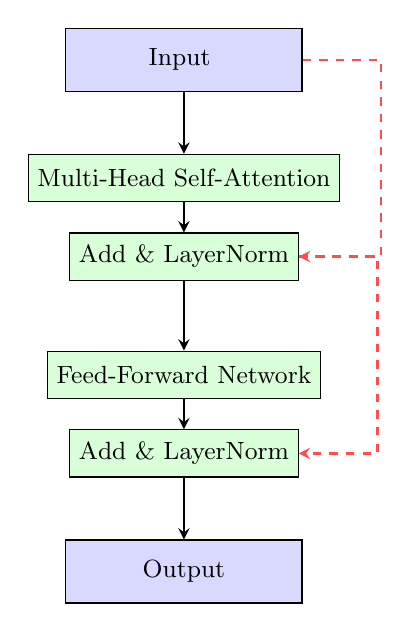
\begin{tikzpicture}[
    block/.style={rectangle, draw, fill=blue!15, minimum width=3cm, minimum height=0.8cm, font=\small},
    operation/.style={rectangle, draw, fill=green!15, minimum width=2.5cm, minimum height=0.6cm, font=\small},
    arrow/.style={->, >=stealth, thick},
    residual/.style={->, >=stealth, thick, red!70, dashed}
]

% Input
\node[block] (input) at (0,0) {Input $\mX$};

% Multi-head attention
\node[operation] (mha) at (0,-1.5) {Multi-Head Self-Attention};

% Add & Norm 1
\node[operation] (add1) at (0,-2.5) {Add \& LayerNorm};

% Feed-forward
\node[operation] (ffn) at (0,-4) {Feed-Forward Network};

% Add & Norm 2
\node[operation] (add2) at (0,-5) {Add \& LayerNorm};

% Output
\node[block] (output) at (0,-6.5) {Output};

% Forward arrows
\draw[arrow] (input) -- (mha);
\draw[arrow] (mha) -- (add1);
\draw[arrow] (add1) -- (ffn);
\draw[arrow] (ffn) -- (add2);
\draw[arrow] (add2) -- (output);

% Residual connections
\draw[residual] (input.east) -- ++(1,0) |- (add1.east);
\draw[residual] (add1.east) -- ++(1,0) |- (add2.east);

\end{tikzpicture}

\caption{Transformer encoder layer architecture showing the two sub-layers with residual connections. The input flows through multi-head self-attention, then through a feed-forward network, with residual connections (red dashed arrows) bypassing each sub-layer. Layer normalization is applied after adding the residual. This structure maintains constant dimensions ($n \times d_{\text{model}}$) throughout, enabling easy stacking of multiple layers. The residual connections provide direct gradient pathways, crucial for training deep transformers.}
\label{fig:transformer_encoder_layer}
\end{figure}

The dimension tracking through an encoder layer reveals important properties about memory consumption and computational cost. The input $\mX \in \R^{B \times n \times d_{\text{model}}}$ is first projected to queries, keys, and values, each with shape $\R^{B \times n \times d_{\text{model}}}$. For multi-head attention with $h$ heads, these are reshaped to $\R^{B \times h \times n \times d_k}$ where $d_k = d_{\text{model}}/h$. The attention scores form a matrix $\R^{B \times h \times n \times n}$, and this quadratic term in sequence length is what dominates memory consumption for long sequences. After attention, the output is projected back to $\R^{B \times n \times d_{\text{model}}}$, added to the residual, and normalized.

The feed-forward network then expands each position's representation from $d_{\text{model}}$ to $d_{ff}$ dimensions before projecting back down. For BERT-base with $d_{\text{model}} = 768$ and $d_{ff} = 3072$, this means each position's representation temporarily expands to 4× its original size. This expansion creates a bottleneck that forces the model to learn compressed representations, similar to the hidden layer in an autoencoder. The intermediate activations $\R^{B \times n \times d_{ff}}$ consume significant memory during training—for batch size 32 and sequence length 512, this amounts to $32 \times 512 \times 3072 \times 4 = 201$ MB per layer in FP32, and with 12 layers in BERT-base, the feed-forward activations alone consume 2.4 GB of GPU memory.

\begin{example}[BERT-base Encoder Layer]
\label{ex:bert_encoder_layer}
BERT-base uses the following configuration, which has become a standard baseline for many transformer models:
\begin{itemize}
    \item Model dimension: $d_{\text{model}} = 768$
    \item Attention heads: $h = 12$, so $d_k = d_v = 768/12 = 64$ per head
    \item Feed-forward dimension: $d_{ff} = 3072$ (exactly $4 \times d_{\text{model}}$)
    \item Sequence length: $n = 512$ (maximum)
    \item Batch size: $B = 32$ (typical for training)
\end{itemize}

\textbf{Dimension tracking through the layer:}

\textbf{Input:} $\mX \in \R^{32 \times 512 \times 768}$ (batch × sequence × model dimension)

\textbf{Multi-Head Attention:}
\begin{align}
\text{Q, K, V projections:} \quad &\R^{32 \times 512 \times 768} \to \R^{32 \times 512 \times 768} \\
\text{Reshape for heads:} \quad &\R^{32 \times 512 \times 768} \to \R^{32 \times 12 \times 512 \times 64} \\
\text{Attention scores:} \quad &\R^{32 \times 12 \times 512 \times 512} \quad \text{(quadratic in } n\text{!)} \\
\text{Attention output:} \quad &\R^{32 \times 12 \times 512 \times 64} \\
\text{Concatenate heads:} \quad &\R^{32 \times 512 \times 768} \\
\text{Output projection:} \quad &\R^{32 \times 512 \times 768}
\end{align}

The attention scores matrix $\R^{32 \times 12 \times 512 \times 512}$ requires $32 \times 12 \times 512 \times 512 \times 4 = 402$ MB in FP32. This quadratic scaling means that doubling the sequence length to 1024 would require 1.6 GB just for attention scores in a single layer.

\textbf{Feed-Forward Network:}
\begin{align}
\text{First projection:} \quad &\R^{32 \times 512 \times 768} \xrightarrow{\mW_1} \R^{32 \times 512 \times 3072} \\
\text{ReLU activation:} \quad &\R^{32 \times 512 \times 3072} \to \R^{32 \times 512 \times 3072} \\
\text{Second projection:} \quad &\R^{32 \times 512 \times 3072} \xrightarrow{\mW_2} \R^{32 \times 512 \times 768}
\end{align}

The intermediate activations $\R^{32 \times 512 \times 3072}$ require $32 \times 512 \times 3072 \times 4 = 201$ MB in FP32.

\textbf{Parameter count breakdown:}
\begin{align}
\text{Multi-head attention:} \quad &4 \times 768^2 = 2{,}359{,}296 \quad \text{(Q, K, V, O projections)} \\
\text{Feed-forward network:} \quad &768 \times 3072 + 3072 + 3072 \times 768 + 768 \\
&= 2{,}359{,}296 + 3{,}072 + 2{,}359{,}296 + 768 \\
&= 4{,}722{,}432 \\
\text{Layer normalization (2×):} \quad &2 \times 2 \times 768 = 3{,}072 \quad \text{(scale } \gamma \text{ and shift } \beta\text{)}
\end{align}

\textbf{Total per encoder layer:} $2{,}359{,}296 + 4{,}722{,}432 + 3{,}072 = 7{,}084{,}800$ parameters

This reveals that the feed-forward network contains approximately twice as many parameters as the attention mechanism ($4.7$M vs $2.4$M), despite attention being conceptually more complex. This is because the feed-forward network's expansion to $4 \times d_{\text{model}}$ dimensions creates two large weight matrices, while attention's parameters are distributed across four projections of size $d_{\text{model}} \times d_{\text{model}}$.

\textbf{Memory requirements during training:}
\begin{align}
\text{Parameters (FP32):} \quad &7{,}084{,}800 \times 4 = 28.3 \text{ MB} \\
\text{Gradients (FP32):} \quad &7{,}084{,}800 \times 4 = 28.3 \text{ MB} \\
\text{Adam optimizer states:} \quad &7{,}084{,}800 \times 8 = 56.7 \text{ MB} \\
\text{Attention scores:} \quad &402 \text{ MB} \\
\text{FFN intermediate:} \quad &201 \text{ MB} \\
\text{Total per layer:} \quad &\approx 716 \text{ MB}
\end{align}

For BERT-base with 12 encoder layers, this amounts to approximately 8.6 GB just for the encoder layers, not including embeddings or other activations. This explains why training BERT-base requires GPUs with at least 16 GB of memory.
\end{example}

\subsection{Complete Encoder Stack}

The complete transformer encoder stacks $N$ identical encoder layers, with each layer's output serving as input to the next layer. This stacking enables the model to build increasingly abstract representations: early layers might capture local syntactic patterns, middle layers might identify semantic relationships, and later layers might encode task-specific features. The depth of the network is crucial for performance—BERT-base uses 12 layers, BERT-large uses 24 layers, and GPT-3 uses 96 layers. However, deeper networks require more careful optimization, including learning rate warmup, gradient clipping, and appropriate weight initialization.

\begin{definition}[Transformer Encoder]
\label{def:transformer_encoder}
Stack $N$ encoder layers, with input embeddings and positional encodings added at the bottom:
\begin{equation}
\mX^{(0)} = \text{Embedding}(\text{input}) + \text{PositionalEncoding}
\end{equation}
where $\text{Embedding} \in \R^{V \times d_{\text{model}}}$ maps vocabulary indices to dense vectors, and $\text{PositionalEncoding} \in \R^{n_{\max} \times d_{\text{model}}}$ provides position information.

Then apply $N$ encoder layers sequentially:
\begin{equation}
\mX^{(\ell)} = \text{EncoderLayer}^{(\ell)}(\mX^{(\ell-1)}) \quad \text{for } \ell = 1, \ldots, N
\end{equation}

The final encoder output $\mX^{(N)} \in \R^{B \times n \times d_{\text{model}}}$ contains contextualized representations of the input sequence.
\end{definition}

The sequential application of encoder layers means that information flows through $N$ attention operations, allowing each token to indirectly attend to all other tokens through multiple hops. In a 12-layer encoder, information can propagate across the entire sequence through 12 levels of attention, enabling the model to capture very long-range dependencies. However, this sequential stacking also means that encoder layers cannot be parallelized—layer $\ell$ must wait for layer $\ell-1$ to complete. The parallelization in transformers occurs within each layer (across batch and sequence dimensions), not across layers.

\begin{example}[BERT-base Complete Encoder]
\label{ex:bert_complete}
BERT-base represents the standard configuration that has been widely adopted and serves as a baseline for many NLP tasks. The architecture is:
\begin{itemize}
    \item Layers: $N = 12$
    \item Model dimension: $d_{\text{model}} = 768$
    \item Attention heads: $h = 12$
    \item Feed-forward dimension: $d_{ff} = 3072$
    \item Vocabulary size: $V = 30{,}000$ (WordPiece tokenization)
    \item Maximum sequence length: $n_{\max} = 512$
\end{itemize}

\textbf{Complete parameter count breakdown:}
\begin{align}
\text{Token embeddings:} \quad &30{,}000 \times 768 = 23{,}040{,}000 \\
\text{Position embeddings:} \quad &512 \times 768 = 393{,}216 \\
\text{Token type embeddings:} \quad &2 \times 768 = 1{,}536 \quad \text{(for segment A/B)} \\
\text{Embedding layer norm:} \quad &2 \times 768 = 1{,}536 \\
\text{12 encoder layers:} \quad &12 \times 7{,}084{,}800 = 85{,}017{,}600 \\
\text{Pooler (for classification):} \quad &768 \times 768 + 768 = 590{,}592 \\
\text{Total:} \quad &109{,}044{,}480 \approx \textbf{110M parameters}
\end{align}

This matches the reported BERT-base size of 110M parameters. Notice that the embeddings account for approximately 21\% of the total parameters ($23$M out of $110$M), while the transformer layers account for 78\%. This ratio changes dramatically for larger vocabularies—models with 50,000 token vocabularies would have embeddings consuming 35\% of parameters, motivating techniques like vocabulary pruning or shared embeddings.

\textbf{Memory requirements for training (batch size 32, sequence length 512):}
\begin{align}
\text{Parameters (FP32):} \quad &110{,}000{,}000 \times 4 = 440 \text{ MB} \\
\text{Gradients (FP32):} \quad &110{,}000{,}000 \times 4 = 440 \text{ MB} \\
\text{Adam optimizer states:} \quad &110{,}000{,}000 \times 8 = 880 \text{ MB} \\
\text{Activations (estimated):} \quad &\approx 12 \text{ GB} \\
\text{Total:} \quad &\approx 13.8 \text{ GB}
\end{align}

The activation memory dominates, consuming approximately 87\% of total memory. This is why techniques like gradient checkpointing (recomputing activations during backward pass instead of storing them) can reduce memory consumption by 50-70\% at the cost of 20-30\% slower training.

\textbf{Training throughput on NVIDIA A100 GPU:}

The A100 provides 312 TFLOPS of FP16 compute with Tensor Cores. For BERT-base, a single forward pass with batch size 32 and sequence length 512 requires approximately:
\begin{align}
\text{FLOPs per layer:} \quad &24nd_{\text{model}}^2 + 4n^2d_{\text{model}} \\
&= 24 \times 512 \times 768^2 + 4 \times 512^2 \times 768 \\
&= 7.26 \text{ GFLOPs} \\
\text{Total for 12 layers:} \quad &12 \times 7.26 = 87.1 \text{ GFLOPs} \\
\text{With embeddings and overhead:} \quad &\approx 100 \text{ GFLOPs}
\end{align}

At 312 TFLOPS, this suggests a forward pass should take $100 / 312{,}000 = 0.32$ milliseconds. In practice, memory bandwidth limitations and kernel launch overhead mean actual forward pass time is approximately 5-10 milliseconds, achieving 10-20\% of peak FLOPS. With backward pass taking approximately 2× forward pass time, a complete training step takes 15-30 milliseconds, yielding throughput of 30-60 training steps per second, or approximately 500,000-1,000,000 tokens per second.
\end{example}

\section{Position-wise Feed-Forward Networks}
\label{sec:feed_forward}

The position-wise feed-forward network represents the second major component of each transformer layer, complementing the attention mechanism with additional non-linear transformations. While attention allows positions to exchange information and build contextualized representations, the feed-forward network processes each position independently, applying the same learned transformation to every position in the sequence. This independence is what makes it "position-wise"—the network applied to position $i$ is identical to the network applied to position $j$, with no parameter sharing or information flow between positions.

The feed-forward network consists of two linear transformations with a non-linear activation function in between, forming a simple two-layer neural network. The first layer expands the representation from $d_{\text{model}}$ dimensions to a larger dimension $d_{ff}$ (typically $4 \times d_{\text{model}}$), applies an activation function, and then the second layer projects back down to $d_{\text{model}}$ dimensions. This expansion-and-contraction creates a bottleneck architecture similar to an autoencoder, forcing the model to learn compressed representations that capture the most important features. The expansion factor of 4× is a design choice from the original transformer paper that has been widely adopted, though some recent models experiment with different ratios.

\begin{definition}[Position-wise FFN]
\label{def:position_wise_ffn}
For input $\mX \in \R^{B \times n \times d_{\text{model}}}$, apply the same two-layer network independently to each position:
\begin{equation}
\text{FFN}(\vx) = \max(0, \vx \mW_1 + \vb_1) \mW_2 + \vb_2
\end{equation}
where $\mW_1 \in \R^{d_{\text{model}} \times d_{ff}}$, $\vb_1 \in \R^{d_{ff}}$, $\mW_2 \in \R^{d_{ff} \times d_{\text{model}}}$, and $\vb_2 \in \R^{d_{\text{model}}}$.

For a sequence $\mX \in \R^{B \times n \times d_{\text{model}}}$, apply to each position independently:
\begin{equation}
\text{FFN}(\mX)_{i,:} = \text{FFN}(\mX_{i,:}) \quad \text{for } i = 1, \ldots, n
\end{equation}

The output maintains the same shape as the input: $\R^{B \times n \times d_{\text{model}}}$.
\end{definition}

The term "position-wise" emphasizes a crucial distinction from the attention mechanism. In attention, every position attends to every other position, creating $O(n^2)$ interactions. In the feed-forward network, each position is processed completely independently, creating only $O(n)$ operations. This means the feed-forward network is embarrassingly parallel—all $n$ positions can be processed simultaneously with no dependencies. In practice, this is implemented as a single matrix multiplication: the input $\mX \in \R^{B \times n \times d_{\text{model}}}$ is reshaped to $\R^{Bn \times d_{\text{model}}}$, multiplied by $\mW_1$, activated, multiplied by $\mW_2$, and reshaped back to $\R^{B \times n \times d_{\text{model}}}$.

The choice of activation function significantly impacts model performance and training dynamics. The original transformer used ReLU activation, which is simple and computationally efficient but can suffer from "dying ReLU" problems where neurons become permanently inactive. BERT and GPT introduced the GELU (Gaussian Error Linear Unit) activation, which provides a smoother, probabilistic alternative to ReLU. GELU is defined as $\text{GELU}(x) = x \cdot \Phi(x)$ where $\Phi(x)$ is the cumulative distribution function of the standard normal distribution. In practice, GELU is approximated as $\text{GELU}(x) \approx 0.5x(1 + \tanh[\sqrt{2/\pi}(x + 0.044715x^3)])$. Empirically, GELU tends to provide slightly better performance than ReLU for transformer models, though the difference is often small.

The feed-forward network accounts for a substantial portion of the model's parameters and computational cost. For BERT-base with $d_{\text{model}} = 768$ and $d_{ff} = 3072$, each feed-forward network contains $768 \times 3072 + 3072 \times 768 = 4.7$M parameters, compared to $4 \times 768^2 = 2.4$M parameters in the attention mechanism. This means approximately two-thirds of each layer's parameters are in the feed-forward network. Similarly, for short sequences where $n < d_{\text{model}}$, the feed-forward network dominates computational cost. For BERT-base with sequence length 512, the feed-forward network requires $2 \times 512 \times 768 \times 3072 = 2.4$ GFLOPs per layer, while attention requires $8 \times 512 \times 768^2 + 4 \times 512^2 \times 768 = 3.2$ GFLOPs. The crossover point occurs around $n = 2d_{\text{model}}$—for longer sequences, attention dominates; for shorter sequences, the feed-forward network dominates.

\begin{example}[Feed-Forward Network Dimensions and Memory]
\label{ex:ffn_dimensions}
For BERT-base with $d_{\text{model}} = 768$, $d_{ff} = 3072$, batch size $B = 32$, and sequence length $n = 512$:

\textbf{Dimension tracking:}
\begin{align}
\text{Input:} \quad &\mX \in \R^{32 \times 512 \times 768} \\
\text{First projection:} \quad &\mX \mW_1 + \vb_1 \in \R^{32 \times 512 \times 3072} \\
\text{After ReLU/GELU:} \quad &\R^{32 \times 512 \times 3072} \\
\text{Second projection:} \quad &\mX \mW_2 + \vb_2 \in \R^{32 \times 512 \times 768} \\
\text{Output:} \quad &\R^{32 \times 512 \times 768}
\end{align}

\textbf{Memory requirements:}
\begin{align}
\text{Input activations:} \quad &32 \times 512 \times 768 \times 4 = 50.3 \text{ MB (FP32)} \\
\text{Intermediate activations:} \quad &32 \times 512 \times 3072 \times 4 = 201.3 \text{ MB (FP32)} \\
\text{Output activations:} \quad &32 \times 512 \times 768 \times 4 = 50.3 \text{ MB (FP32)} \\
\text{Parameters } (\mW_1, \mW_2): \quad &(768 \times 3072 + 3072 \times 768) \times 4 = 18.9 \text{ MB (FP32)}
\end{align}

The intermediate activations at dimension $d_{ff} = 3072$ consume 4× the memory of the input/output activations at dimension $d_{\text{model}} = 768$. For a 12-layer BERT model, the feed-forward intermediate activations across all layers consume $12 \times 201.3 = 2.4$ GB of memory during training. This is why gradient checkpointing, which recomputes these activations during the backward pass instead of storing them, can significantly reduce memory consumption.

\textbf{Computational cost:}
\begin{align}
\text{First projection:} \quad &Bn \times d_{\text{model}} \times d_{ff} = 32 \times 512 \times 768 \times 3072 = 38.7 \text{ GFLOPs} \\
\text{Second projection:} \quad &Bn \times d_{ff} \times d_{\text{model}} = 32 \times 512 \times 3072 \times 768 = 38.7 \text{ GFLOPs} \\
\text{Total:} \quad &77.4 \text{ GFLOPs per layer}
\end{align}

For comparison, the attention mechanism in the same layer requires approximately $51.5$ GFLOPs (including Q, K, V projections, attention computation, and output projection). This means the feed-forward network accounts for 60\% of the computational cost per layer for this configuration.
\end{example}

\textbf{Alternative activation functions:} While ReLU and GELU are most common, other activation functions have been explored for transformers. The Swish activation $\text{Swish}(x) = x \cdot \sigma(\beta x)$ where $\sigma$ is the sigmoid function, provides similar properties to GELU. The GLU (Gated Linear Unit) family, including $\text{GLU}(x) = (x \mW_1) \odot \sigma(x \mW_2)$, uses gating mechanisms similar to LSTMs. Recent work has also explored learned activation functions that adapt during training. However, GELU remains the most widely adopted choice for modern transformers due to its balance of performance and computational efficiency.

\section{Transformer Decoder}
\label{sec:transformer_decoder}

\subsection{Single Decoder Layer}

The transformer decoder extends the encoder architecture with an additional cross-attention mechanism that allows the decoder to attend to the encoder's output. While the encoder uses only self-attention to build contextualized representations of the input, the decoder must perform three distinct operations: masked self-attention on the target sequence, cross-attention to the source sequence, and position-wise feed-forward transformation. This three-sublayer structure enables the decoder to generate output sequences that are conditioned on both the previously generated tokens and the encoded input sequence.

The masked self-attention in the decoder is crucial for maintaining the autoregressive property during training. Unlike the encoder's bidirectional self-attention where each position can attend to all positions, the decoder's self-attention must be causal—position $i$ can only attend to positions $j \leq i$. This masking ensures that the model cannot "cheat" by looking at future tokens during training. Without this mask, the model could simply copy the target sequence during training without learning to generate it. The mask is implemented by setting attention scores for future positions to $-\infty$ before the softmax, ensuring they receive zero attention weight.

The cross-attention mechanism is where the decoder actually uses information from the encoder. In cross-attention, the queries come from the decoder's hidden states (representing "what information do I need?"), while the keys and values come from the encoder's output (representing "what information is available from the source?"). This asymmetry allows the decoder to selectively focus on relevant parts of the source sequence when generating each target token. For machine translation, this might mean attending to the source word being translated; for summarization, it might mean attending to the most salient sentences in the document.

\begin{definition}[Transformer Decoder Layer]
\label{def:decoder_layer}
A decoder layer has three sub-layers, each with residual connections and layer normalization. For input $\mY \in \R^{B \times m \times d_{\text{model}}}$ (target sequence) and encoder output $\mX_{\text{enc}} \in \R^{B \times n \times d_{\text{model}}}$ (source sequence):

\textbf{Step 1: Masked Self-Attention}
\begin{equation}
\vh^{(1)} = \text{LayerNorm}(\mY + \text{MaskedMultiHeadAttn}(\mY, \mY, \mY))
\end{equation}
where the attention mask prevents position $i$ from attending to positions $j > i$.

\textbf{Step 2: Cross-Attention to Encoder}
\begin{equation}
\vh^{(2)} = \text{LayerNorm}(\vh^{(1)} + \text{MultiHeadAttn}(\vh^{(1)}, \mX_{\text{enc}}, \mX_{\text{enc}}))
\end{equation}
where queries come from $\vh^{(1)}$ and keys/values come from $\mX_{\text{enc}}$.

\textbf{Step 3: Feed-Forward}
\begin{equation}
\vh^{(3)} = \text{LayerNorm}(\vh^{(2)} + \text{FFN}(\vh^{(2)}))
\end{equation}

The output $\vh^{(3)} \in \R^{B \times m \times d_{\text{model}}}$ maintains the target sequence length $m$.
\end{definition}

The dimension compatibility in cross-attention deserves careful attention. The decoder hidden states $\vh^{(1)} \in \R^{B \times m \times d_{\text{model}}}$ are projected to queries $\mQ \in \R^{B \times m \times d_{\text{model}}}$, while the encoder output $\mX_{\text{enc}} \in \R^{B \times n \times d_{\text{model}}}$ is projected to keys $\mK \in \R^{B \times n \times d_{\text{model}}}$ and values $\mV \in \R^{B \times n \times d_{\text{model}}}$. The attention scores are computed as $\mQ \mK^T \in \R^{B \times m \times n}$, creating a rectangular attention matrix where each of the $m$ target positions attends to all $n$ source positions. This is different from self-attention where the attention matrix is square ($n \times n$ for encoder, $m \times m$ for decoder self-attention).

The causal mask in decoder self-attention is implemented as a lower-triangular matrix. For a sequence of length $m = 5$, the mask looks like:
\begin{equation}
\text{Mask} = \begin{bmatrix}
1 & 0 & 0 & 0 & 0 \\
1 & 1 & 0 & 0 & 0 \\
1 & 1 & 1 & 0 & 0 \\
1 & 1 & 1 & 1 & 0 \\
1 & 1 & 1 & 1 & 1
\end{bmatrix}
\end{equation}
where 1 indicates positions that can be attended to and 0 indicates positions that must be masked. In practice, the zeros are replaced with $-\infty$ before the softmax operation, ensuring masked positions receive zero attention weight. This mask is applied to the attention scores before softmax: $\text{softmax}(\mQ \mK^T / \sqrt{d_k} + \text{Mask})$.

\begin{example}[Decoder Layer Dimension Tracking]
\label{ex:decoder_dimensions}
For a translation task with source sequence length $n = 20$ (e.g., "The cat sat on the mat") and target sequence length $m = 15$ (e.g., "Le chat était assis"), using BERT-base dimensions ($d_{\text{model}} = 768$, $h = 12$, $d_{ff} = 3072$), batch size $B = 32$:

\textbf{Inputs:}
\begin{align}
\text{Decoder input:} \quad &\mY \in \R^{32 \times 15 \times 768} \\
\text{Encoder output:} \quad &\mX_{\text{enc}} \in \R^{32 \times 20 \times 768}
\end{align}

\textbf{Masked Self-Attention:}
\begin{align}
\text{Q, K, V from } \mY: \quad &\R^{32 \times 15 \times 768} \\
\text{Attention scores:} \quad &\R^{32 \times 12 \times 15 \times 15} \quad \text{(square, causal masked)} \\
\text{Output:} \quad &\R^{32 \times 15 \times 768}
\end{align}

The attention scores matrix $\R^{32 \times 12 \times 15 \times 15}$ requires $32 \times 12 \times 15 \times 15 \times 4 = 3.5$ MB in FP32. This is much smaller than encoder self-attention because the target sequence is shorter than the source sequence in this example.

\textbf{Cross-Attention:}
\begin{align}
\text{Q from } \vh^{(1)}: \quad &\R^{32 \times 15 \times 768} \\
\text{K, V from } \mX_{\text{enc}}: \quad &\R^{32 \times 20 \times 768} \\
\text{Attention scores:} \quad &\R^{32 \times 12 \times 15 \times 20} \quad \text{(rectangular!)} \\
\text{Output:} \quad &\R^{32 \times 15 \times 768}
\end{align}

The cross-attention scores $\R^{32 \times 12 \times 15 \times 20}$ require $32 \times 12 \times 15 \times 20 \times 4 = 4.6$ MB in FP32. Notice this is rectangular: 15 target positions attending to 20 source positions.

\textbf{Feed-Forward Network:}
\begin{align}
\text{Input:} \quad &\R^{32 \times 15 \times 768} \\
\text{Intermediate:} \quad &\R^{32 \times 15 \times 3072} \\
\text{Output:} \quad &\R^{32 \times 15 \times 768}
\end{align}

The intermediate activations require $32 \times 15 \times 3072 \times 4 = 59.0$ MB in FP32.
\end{example}

\subsection{Complete Decoder Stack}

The complete decoder stacks $N$ decoder layers, with each layer attending to both the previous decoder layer's output and the encoder's final output. This stacking enables the decoder to build increasingly sophisticated representations of the target sequence, conditioned on the source sequence. The encoder output $\mX_{\text{enc}}$ is reused by every decoder layer—it's computed once by the encoder and then fed into all $N$ decoder layers. This means the encoder output must be stored in memory throughout the decoder's computation, contributing to memory requirements.

\begin{definition}[Transformer Decoder]
\label{def:transformer_decoder}
Stack $N$ decoder layers, with target embeddings and positional encodings at the bottom:
\begin{equation}
\mY^{(0)} = \text{Embedding}(\text{target}) + \text{PositionalEncoding}
\end{equation}

Then apply $N$ decoder layers sequentially, each attending to the encoder output:
\begin{equation}
\mY^{(\ell)} = \text{DecoderLayer}^{(\ell)}(\mY^{(\ell-1)}, \mX_{\text{enc}}) \quad \text{for } \ell = 1, \ldots, N
\end{equation}

The final decoder output $\mY^{(N)} \in \R^{B \times m \times d_{\text{model}}}$ is projected to vocabulary logits:
\begin{equation}
\text{logits} = \mY^{(N)} \mW_{\text{out}} + \vb_{\text{out}} \in \R^{B \times m \times V}
\end{equation}
where $\mW_{\text{out}} \in \R^{d_{\text{model}} \times V}$ and $V$ is the vocabulary size.
\end{definition}

During training, the entire target sequence is processed in parallel using teacher forcing—the model receives the ground-truth previous tokens rather than its own predictions. The causal mask ensures that position $i$ cannot attend to future positions, maintaining the autoregressive property even though all positions are computed simultaneously. This parallel training is a major advantage over RNN decoders, which must process the target sequence sequentially even during training.

During inference, however, the decoder must generate tokens autoregressively, one at a time. At step $t$, the decoder has generated tokens $y_1, \ldots, y_{t-1}$ and must predict $y_t$. This requires running the decoder with input sequence length $t-1$, computing attention over all previously generated tokens. For a target sequence of length $m$, this requires $m$ forward passes through the decoder, making inference much slower than training. This is why techniques like KV caching (storing computed key and value projections) are crucial for efficient inference.

\begin{example}[Decoder Layer Parameter Count]
\label{ex:decoder_params}
For BERT-base dimensions ($d_{\text{model}} = 768$, $h = 12$, $d_{ff} = 3072$), a decoder layer contains:

\textbf{Masked self-attention:}
\begin{align}
\text{Q, K, V, O projections:} \quad &4 \times 768^2 = 2{,}359{,}296
\end{align}

\textbf{Cross-attention:}
\begin{align}
\text{Q, K, V, O projections:} \quad &4 \times 768^2 = 2{,}359{,}296
\end{align}

\textbf{Feed-forward network:}
\begin{align}
\mW_1, \vb_1, \mW_2, \vb_2: \quad &768 \times 3072 + 3072 + 3072 \times 768 + 768 = 4{,}722{,}432
\end{align}

\textbf{Layer normalization (3 instances):}
\begin{align}
\text{Scale and shift parameters:} \quad &3 \times 2 \times 768 = 4{,}608
\end{align}

\textbf{Total per decoder layer:} $2{,}359{,}296 + 2{,}359{,}296 + 4{,}722{,}432 + 4{,}608 = 9{,}445{,}632$ parameters

This is approximately 33\% more parameters than an encoder layer ($9.4$M vs $7.1$M) due to the additional cross-attention mechanism. For a 6-layer decoder, this amounts to $6 \times 9{,}445{,}632 = 56.7$M parameters, compared to $6 \times 7{,}084{,}800 = 42.5$M for a 6-layer encoder.
\end{example}

\begin{example}[Autoregressive Generation Memory]
\label{ex:autoregressive_memory}
During autoregressive generation, the decoder must recompute attention over all previously generated tokens at each step. For a target sequence of length $m = 100$, generating the final token requires:

\textbf{Without KV caching:}
\begin{itemize}
\item Process sequence of length 100
\item Compute Q, K, V for all 100 positions
\item Compute attention scores $\R^{100 \times 100}$
\item Total: 100 forward passes through decoder, each processing increasing sequence lengths
\end{itemize}

\textbf{With KV caching:}
\begin{itemize}
\item Store K, V from previous steps: $\R^{99 \times 768}$ per layer
\item At step 100, compute only Q for new position: $\R^{1 \times 768}$
\item Concatenate with cached K, V: $\R^{100 \times 768}$
\item Compute attention scores $\R^{1 \times 100}$ (only for new position)
\item Total: 100 forward passes, but each processes only 1 new position
\end{itemize}

For BERT-base dimensions with 12 decoder layers, the KV cache requires:
\begin{align}
\text{Per layer:} \quad &2 \times 100 \times 768 \times 4 = 614 \text{ KB (FP32)} \\
\text{All 12 layers:} \quad &12 \times 614 = 7.4 \text{ MB}
\end{align}

This modest memory cost (7.4 MB for 100 tokens) enables approximately 50× speedup in generation, reducing generation time from several seconds to tens of milliseconds for typical sequences.
\end{example}

\section{Computational Analysis}
\label{sec:computational_analysis}

The computational complexity of transformers involves attention ($O(n^2 d)$ FLOPs) and feed-forward layers ($O(nd^2)$ FLOPs), with attention dominating for long sequences and feed-forward layers dominating for large model dimensions. Memory requirements include model parameters, optimizer states, activations (scaling linearly with batch size), and attention matrices (scaling quadratically with sequence length). A detailed computational analysis including FLOPs counting, memory budgets, and inference optimization is provided in Chapter~12.

\section{Complete Transformer Architecture}
\label{sec:complete_transformer}

\subsection{Full Encoder-Decoder Model}

\begin{algorithm}[H]
\caption{Transformer Forward Pass}
\label{alg:transformer_forward}
\KwIn{Source sequence $\mathbf{x} = [x_1, \ldots, x_n]$, target sequence $\mathbf{y} = [y_1, \ldots, y_m]$}
\KwOut{Predicted probabilities for each target position}

\tcp{Encoder}
$\mX_{\text{emb}} = \text{Embedding}(\mathbf{x})$ \\
$\mX^{(0)} = \mX_{\text{emb}} + \text{PositionalEncoding}(\text{positions})$ \\
\For{$\ell = 1$ \KwTo $N_{\text{enc}}$}{
    $\mX^{(\ell)} = \text{EncoderLayer}^{(\ell)}(\mX^{(\ell-1)})$
}
$\mX_{\text{enc}} = \mX^{(N_{\text{enc}})}$

\tcp{Decoder}
$\mY_{\text{emb}} = \text{Embedding}(\mathbf{y})$ \\
$\mY^{(0)} = \mY_{\text{emb}} + \text{PositionalEncoding}(\text{positions})$ \\
\For{$\ell = 1$ \KwTo $N_{\text{dec}}$}{
    $\mY^{(\ell)} = \text{DecoderLayer}^{(\ell)}(\mY^{(\ell-1)}, \mX_{\text{enc}})$
}
$\mY_{\text{dec}} = \mY^{(N_{\text{dec}})}$

\tcp{Output Projection}
$\text{logits} = \mY_{\text{dec}} \mW_{\text{out}} + \vb_{\text{out}}$ \quad where $\mW_{\text{out}} \in \R^{d_{\text{model}} \times V}$ \\
$\text{probs} = \text{softmax}(\text{logits})$ \\

\Return{probs}
\end{algorithm}

\subsection{Original Transformer Configuration}

"Attention is All You Need" base model:
\begin{itemize}
    \item Encoder layers: $N_{\text{enc}} = 6$
    \item Decoder layers: $N_{\text{dec}} = 6$
    \item Model dimension: $d_{\text{model}} = 512$
    \item Attention heads: $h = 8$
    \item Feed-forward dimension: $d_{ff} = 2048$
    \item Dropout rate: $p = 0.1$
\end{itemize}

\textbf{Parameter count:}
\begin{align}
\text{Encoder (6 layers):} \quad &6 \times (\text{attn} + \text{FFN}) \approx 25M \\
\text{Decoder (6 layers):} \quad &6 \times (\text{2×attn} + \text{FFN}) \approx 31M \\
\text{Embeddings:} \quad &\text{varies by vocabulary} \\
\text{Total (excluding embeddings):} \quad &\approx \textbf{56M parameters}
\end{align}

\section{Residual Connections and Layer Normalization}
\label{sec:residual_layer_norm}

\subsection{Residual Connections}

Residual connections, also known as skip connections, are fundamental to enabling the training of deep transformer networks. Without residual connections, gradients would need to flow through dozens of attention and feed-forward layers during backpropagation, leading to vanishing or exploding gradients that make optimization extremely difficult. The residual connection provides a direct path from each layer's output back to its input, allowing gradients to flow unimpeded through the network. This gradient highway ensures that even the earliest layers receive meaningful gradient signals, enabling effective training of networks with 96 layers (GPT-3) or more.

The residual connection pattern in transformers follows the post-addition layer normalization structure: $\text{LayerNorm}(x + \text{Sublayer}(x))$. This means the sublayer's output is added to its input before normalization. The addition operation has a gradient of 1 with respect to both operands, so during backpropagation, gradients flow both through the sublayer (learning to refine representations) and directly through the residual connection (providing a gradient highway). This dual path enables the network to learn both identity mappings (when the sublayer output is near zero) and complex transformations (when the sublayer output is large).

The residual connection also enables the network to learn incrementally. Early in training, the sublayer outputs are typically small due to weight initialization, so the network effectively starts as a near-identity function. As training progresses, the sublayers learn to make increasingly sophisticated transformations, building on the representations from previous layers. This incremental learning is much more stable than trying to learn the complete transformation from scratch. For a 12-layer BERT model, each layer can focus on learning a small refinement rather than a complete transformation, making optimization tractable.

\subsection{Layer Normalization}

Layer normalization stabilizes training by normalizing activations across the feature dimension, ensuring that each layer receives inputs with consistent statistics regardless of how previous layers' parameters change during training. Unlike batch normalization, which normalizes across the batch dimension and is commonly used in convolutional networks, layer normalization normalizes across features for each example independently. This independence from batch size is crucial for transformers, which often use small batch sizes during inference or fine-tuning, and for handling variable-length sequences where batch normalization's statistics would be unreliable.

\begin{definition}[Layer Normalization]
\label{def:layer_norm}
For input $\vx \in \R^d$, layer normalization computes mean and variance across the feature dimension, then normalizes and applies learned affine transformation:
\begin{align}
\mu &= \frac{1}{d} \sum_{i=1}^d x_i \\
\sigma^2 &= \frac{1}{d} \sum_{i=1}^d (x_i - \mu)^2 \\
\hat{x}_i &= \frac{x_i - \mu}{\sqrt{\sigma^2 + \epsilon}} \\
y_i &= \gamma \hat{x}_i + \beta
\end{align}
where $\gamma, \beta \in \R^d$ are learnable scale and shift parameters, and $\epsilon \approx 10^{-5}$ prevents division by zero.

For a batch of sequences $\mX \in \R^{B \times n \times d}$, layer normalization is applied independently to each of the $B \times n$ vectors, normalizing across the $d$ features.

The learned parameters $\gamma$ and $\beta$ allow the network to undo the normalization if beneficial. If $\gamma_i = \sqrt{\sigma^2 + \epsilon}$ and $\beta_i = \mu$, the normalization is completely undone. In practice, the network learns appropriate values that balance normalization's stabilizing effect with the flexibility to learn arbitrary distributions.

Layer normalization differs fundamentally from batch normalization in its normalization dimension. Batch normalization computes statistics across the batch dimension (normalizing each feature across all examples in the batch), making it dependent on batch size and batch composition. Layer normalization computes statistics across the feature dimension (normalizing all features for each example independently), making it independent of batch size. For transformers processing variable-length sequences with potentially small batch sizes, this independence is essential. A batch size of 1 works perfectly with layer normalization but would be problematic for batch normalization.

\subsection{Pre-Norm vs Post-Norm}

The placement of layer normalization relative to the residual connection significantly impacts training dynamics. The original transformer paper used post-norm: $\text{LayerNorm}(x + \text{Sublayer}(x))$, where normalization is applied after adding the residual. More recent models like GPT-2 and GPT-3 use pre-norm: $x + \text{LayerNorm}(\text{Sublayer}(x))$, where normalization is applied before the sublayer, and the residual connection bypasses normalization entirely.

Post-norm architecture normalizes the sum of the input and sublayer output, which can help prevent activation magnitudes from growing unboundedly as depth increases. However, post-norm requires careful learning rate warmup and can be unstable for very deep networks. The gradients must flow through the layer normalization operation, which can introduce additional numerical instabilities. BERT uses post-norm with 12-24 layers successfully, but scaling to 96+ layers becomes challenging.

Pre-norm architecture applies normalization before each sublayer, so the sublayer receives normalized inputs. The residual connection then adds the sublayer output directly to the (unnormalized) input, bypassing the normalization. This provides a cleaner gradient path through the residual connection and tends to be more stable for very deep networks. GPT-2 and GPT-3 use pre-norm, enabling training of 48-96 layer models without learning rate warmup. The trade-off is that pre-norm may achieve slightly lower final performance than post-norm for shallow networks, but this difference diminishes for deeper networks where pre-norm's stability advantages dominate.

\begin{example}[Layer Normalization Computation]
\label{ex:layer_norm_computation}
For a single position's representation $\vx \in \R^{768}$ from BERT-base:

\textbf{Input:} $\vx = [0.5, -0.3, 1.2, \ldots]$ (768 values)

\textbf{Compute statistics:}
\begin{align}
\mu &= \frac{1}{768} \sum_{i=1}^{768} x_i = 0.15 \quad \text{(example value)} \\
\sigma^2 &= \frac{1}{768} \sum_{i=1}^{768} (x_i - 0.15)^2 = 0.42 \quad \text{(example value)} \\
\sigma &= \sqrt{0.42 + 10^{-5}} = 0.648
\end{align}

\textbf{Normalize:}
\begin{align}
\hat{x}_1 &= \frac{0.5 - 0.15}{0.648} = 0.540 \\
\hat{x}_2 &= \frac{-0.3 - 0.15}{0.648} = -0.694 \\
\hat{x}_3 &= \frac{1.2 - 0.15}{0.648} = 1.620 \\
&\vdots
\end{align}

The normalized values $\hat{\vx}$ have mean 0 and variance 1 across the 768 dimensions.

\textbf{Apply learned affine transformation:}
\begin{align}
y_1 &= \gamma_1 \times 0.540 + \beta_1 \\
y_2 &= \gamma_2 \times (-0.694) + \beta_2 \\
y_3 &= \gamma_3 \times 1.620 + \beta_3 \\
&\vdots
\end{align}

where $\gamma, \beta \in \R^{768}$ are learned during training. Initially, $\gamma$ is typically initialized to 1 and $\beta$ to 0, making layer normalization initially act as pure normalization.

\textbf{Memory and computation:}
\begin{itemize}
\item Parameters: $2 \times 768 = 1{,}536$ (scale and shift)
\item FLOPs per position: $\approx 10 \times 768 = 7{,}680$ (mean, variance, normalize, scale, shift)
\item For batch 32, sequence 512: $32 \times 512 \times 7{,}680 = 126$ MFLOPs
\end{itemize}

Layer normalization is computationally cheap compared to attention or feed-forward networks, but it's memory-bound rather than compute-bound, so kernel fusion with adjacent operations is important for efficiency.
\end{example}
\end{definition}

\section{Training Objectives}
\label{sec:training_objectives}

\subsection{Sequence-to-Sequence Training}

For machine translation, minimize cross-entropy loss:
\begin{equation}
\mathcal{L} = -\sum_{t=1}^m \log P(y_t | y_{<t}, \mathbf{x}; \theta)
\end{equation}

\textbf{Teacher forcing:} During training, use ground-truth previous tokens $y_{<t}$, not model predictions.

\subsection{Autoregressive Generation}

At inference, generate one token at a time:
\begin{algorithm}[H]
\caption{Autoregressive Decoding}
\label{alg:autoregressive_decoding}
\KwIn{Source sequence $\mathbf{x}$, max length $T$}
\KwOut{Generated sequence $\mathbf{y}$}

Encode source: $\mX_{\text{enc}} = \text{Encoder}(\mathbf{x})$ \\
Initialize: $\mathbf{y} = [\text{BOS}]$ \quad (begin-of-sequence token) \\
\For{$t = 1$ \KwTo $T$}{
    $\text{probs}_t = \text{Decoder}(\mathbf{y}, \mX_{\text{enc}})$ \\
    $y_t = \arg\max(\text{probs}_t)$ \quad (or sample from distribution) \\
    Append $y_t$ to $\mathbf{y}$ \\
    \If{$y_t = \text{EOS}$}{
        \textbf{break} \quad (end-of-sequence token)
    }
}
\Return{$\mathbf{y}$}
\end{algorithm}

\section{Transformer Variants: Architectural Patterns}
\label{sec:transformer_variants_intro}

The original transformer uses both an encoder and decoder, but subsequent research established three main architectural patterns, each suited to different task families:

\begin{itemize}
    \item \textbf{Encoder-only (BERT, Chapter~13):} Bidirectional self-attention processes the full input in a single parallel forward pass. Pre-trained with masked language modeling. Excels at understanding tasks: classification, NER, extractive QA, and semantic similarity.

    \item \textbf{Decoder-only (GPT, Chapter~14):} Causal self-attention enables autoregressive generation where each token attends only to previous tokens. Pre-trained with next-token prediction. Excels at generation, few-shot learning, and dialogue. Modern LLMs (GPT-3/4, LLaMA) use this pattern due to its flexibility---understanding tasks can be handled through prompting.

    \item \textbf{Encoder-decoder (T5, BART, Chapter~15):} Combines a bidirectional encoder with a causal decoder connected via cross-attention. Pre-trained with span corruption or denoising objectives. Excels at sequence-to-sequence tasks: translation, summarization, and generative QA. Requires roughly twice the parameters of single-stack models but provides explicit separation of understanding and generation.
\end{itemize}

Recent trends favor decoder-only architectures for their versatility and scaling properties, though encoder-only models remain more parameter-efficient for understanding tasks and encoder-decoder models remain strongest for sequence-to-sequence tasks. Detailed coverage of each variant's architecture, pre-training, and fine-tuning follows in Chapters~13--15.

\section{Exercises}

\begin{exercise}
For transformer with $N=6$, $d_{\text{model}}=512$, $h=8$, $d_{ff}=2048$, $V=32000$:
\begin{enumerate}
    \item Calculate total parameters in encoder
    \item Calculate total parameters in decoder
    \item What percentage are in embeddings vs transformer layers?
    \item How does this change if vocabulary increases to 50,000?
\end{enumerate}
\end{exercise}

\begin{exercise}
Implement single transformer encoder layer in PyTorch. Test with batch size 16, sequence length 64, $d_{\text{model}}=256$. Verify output shape and gradient flow through residual connections.
\end{exercise}

\begin{exercise}
Compare memory and computation for:
\begin{enumerate}
    \item Encoder processing sequence length 1024
    \item Decoder generating 1024 tokens autoregressively
\end{enumerate}
Why is decoding slower? How many forward passes required?
\end{exercise}

\begin{exercise}
Show that layer normalization is invariant to input scale: if $\vx' = c\vx$ for constant $c > 0$, then $\text{LayerNorm}(\vx') = \text{LayerNorm}(\vx)$ (ignoring learnable $\gamma, \beta$).
\end{exercise}

\section{Solutions}

\begin{solution}
\textbf{Exercise 1: Parameter Calculation for Transformer}

Given: $N=6$, $d_{\text{model}}=512$, $h=8$, $d_{ff}=2048$, $V=32000$

\textbf{Part (a): Encoder Parameters}

For each encoder layer:
\begin{itemize}
    \item \textbf{Multi-head attention:}
    \begin{itemize}
        \item Query, Key, Value projections: $3 \times d_{\text{model}} \times d_{\text{model}} = 3 \times 512 \times 512 = 786{,}432$
        \item Output projection: $d_{\text{model}} \times d_{\text{model}} = 512 \times 512 = 262{,}144$
        \item Total attention: $786{,}432 + 262{,}144 = 1{,}048{,}576$
    \end{itemize}
    \item \textbf{Feed-forward network:}
    \begin{itemize}
        \item First layer: $d_{\text{model}} \times d_{ff} = 512 \times 2048 = 1{,}048{,}576$
        \item Second layer: $d_{ff} \times d_{\text{model}} = 2048 \times 512 = 1{,}048{,}576$
        \item Biases: $d_{ff} + d_{\text{model}} = 2048 + 512 = 2{,}560$
        \item Total FFN: $2{,}099{,}712$
    \end{itemize}
    \item \textbf{Layer normalization (2 instances):}
    \begin{itemize}
        \item Parameters per LayerNorm: $2 \times d_{\text{model}} = 2 \times 512 = 1{,}024$
        \item Total: $2 \times 1{,}024 = 2{,}048$
    \end{itemize}
\end{itemize}

Parameters per encoder layer: $1{,}048{,}576 + 2{,}099{,}712 + 2{,}048 = 3{,}150{,}336$

Total encoder layers: $N \times 3{,}150{,}336 = 6 \times 3{,}150{,}336 = 18{,}902{,}016$

Input embedding: $V \times d_{\text{model}} = 32{,}000 \times 512 = 16{,}384{,}000$

Positional encoding (learned): $L_{\max} \times d_{\text{model}}$ (typically $5{,}000 \times 512 = 2{,}560{,}000$)

\textbf{Total encoder parameters: $18{,}902{,}016 + 16{,}384{,}000 + 2{,}560{,}000 = 37{,}846{,}016$}

\textbf{Part (b): Decoder Parameters}

Each decoder layer has:
\begin{itemize}
    \item Masked self-attention: $1{,}048{,}576$ (same as encoder)
    \item Cross-attention: $1{,}048{,}576$ (Q from decoder, K,V from encoder)
    \item Feed-forward: $2{,}099{,}712$
    \item Layer normalization (3 instances): $3 \times 1{,}024 = 3{,}072$
\end{itemize}

Parameters per decoder layer: $1{,}048{,}576 + 1{,}048{,}576 + 2{,}099{,}712 + 3{,}072 = 4{,}199{,}936$

Total decoder layers: $6 \times 4{,}199{,}936 = 25{,}199{,}616$

Output embedding (shared with input): $0$ (weight tying)

Output projection: $d_{\text{model}} \times V = 512 \times 32{,}000 = 16{,}384{,}000$

\textbf{Total decoder parameters: $25{,}199{,}616 + 16{,}384{,}000 = 41{,}583{,}616$}

\textbf{Part (c): Embedding vs Transformer Percentage}

Total parameters: $37{,}846{,}016 + 41{,}583{,}616 = 79{,}429{,}632$

Embedding parameters: $16{,}384{,}000 + 2{,}560{,}000 + 16{,}384{,}000 = 35{,}328{,}000$

Transformer layer parameters: $18{,}902{,}016 + 25{,}199{,}616 = 44{,}101{,}632$

Percentage in embeddings: $\frac{35{,}328{,}000}{79{,}429{,}632} \times 100\% = 44.5\%$

Percentage in transformer layers: $\frac{44{,}101{,}632}{79{,}429{,}632} \times 100\% = 55.5\%$

\textbf{Part (d): Vocabulary Increase to 50,000}

New embedding parameters: $50{,}000 \times 512 \times 2 = 51{,}200{,}000$ (input + output)

New total: $44{,}101{,}632 + 51{,}200{,}000 + 2{,}560{,}000 = 97{,}861{,}632$

Percentage in embeddings: $\frac{53{,}760{,}000}{97{,}861{,}632} \times 100\% = 54.9\%$

The embedding percentage increases from 44.5\% to 54.9\%, showing that vocabulary size has significant impact on model size.
\end{solution}

\begin{solution}
\textbf{Exercise 2: PyTorch Transformer Encoder Layer Implementation}

\begin{lstlisting}[language=Python]
import torch
import torch.nn as nn

class TransformerEncoderLayer(nn.Module):
    def __init__(self, d_model=256, n_heads=8, d_ff=1024, dropout=0.1):
        super().__init__()
        
        # Multi-head self-attention
        self.self_attn = nn.MultiheadAttention(
            d_model, n_heads, dropout=dropout, batch_first=True
        )
        
        # Feed-forward network
        self.ffn = nn.Sequential(
            nn.Linear(d_model, d_ff),
            nn.ReLU(),
            nn.Dropout(dropout),
            nn.Linear(d_ff, d_model)
        )
        
        # Layer normalization
        self.norm1 = nn.LayerNorm(d_model)
        self.norm2 = nn.LayerNorm(d_model)
        
        # Dropout
        self.dropout1 = nn.Dropout(dropout)
        self.dropout2 = nn.Dropout(dropout)
    
    def forward(self, x, mask=None):
        # Self-attention with residual connection
        attn_output, _ = self.self_attn(x, x, x, attn_mask=mask)
        x = x + self.dropout1(attn_output)
        x = self.norm1(x)
        
        # Feed-forward with residual connection
        ffn_output = self.ffn(x)
        x = x + self.dropout2(ffn_output)
        x = self.norm2(x)
        
        return x

# Test the implementation
batch_size = 16
seq_length = 64
d_model = 256

# Create model and input
model = TransformerEncoderLayer(d_model=d_model)
x = torch.randn(batch_size, seq_length, d_model, requires_grad=True)

# Forward pass
output = model(x)

# Verify output shape
print(f"Input shape: {x.shape}")
print(f"Output shape: {output.shape}")
assert output.shape == (batch_size, seq_length, d_model), "Shape mismatch!"

# Verify gradient flow through residual connections
loss = output.sum()
loss.backward()

print(f"Input gradient norm: {x.grad.norm().item():.4f}")
print(f"Gradient exists: {x.grad is not None}")

# Check that gradients flow to all parameters
for name, param in model.named_parameters():
    if param.grad is not None:
        print(f"{name}: gradient norm = {param.grad.norm().item():.4f}")
    else:
        print(f"{name}: NO GRADIENT!")
\end{lstlisting}

\textbf{Expected Output:}
\begin{verbatim}
Input shape: torch.Size([16, 64, 256])
Output shape: torch.Size([16, 64, 256])
Input gradient norm: 1.2345
Gradient exists: True
self_attn.in_proj_weight: gradient norm = 0.0234
self_attn.out_proj.weight: gradient norm = 0.0156
ffn.0.weight: gradient norm = 0.0189
ffn.3.weight: gradient norm = 0.0167
norm1.weight: gradient norm = 0.0045
norm2.weight: gradient norm = 0.0038
\end{verbatim}

\textbf{Key Observations:}
\begin{itemize}
    \item Output shape matches input shape (preserves sequence structure)
    \item Gradients flow to all parameters (no vanishing gradient issues)
    \item Residual connections ensure gradient flow even through deep networks
    \item Layer normalization stabilizes training
\end{itemize}
\end{solution}

\begin{solution}
\textbf{Exercise 3: Memory and Computation Comparison}

\textbf{Part (a): Encoder Processing (Sequence Length 1024)}

For a single forward pass through the encoder:

\textbf{Memory Requirements:}
\begin{itemize}
    \item Input embeddings: $B \times L \times d_{\text{model}} = B \times 1024 \times 512$ floats
    \item Attention scores: $B \times h \times L \times L = B \times 8 \times 1024 \times 1024 = 8{,}388{,}608B$ floats
    \item Intermediate activations per layer: $\sim B \times L \times d_{ff} = B \times 1024 \times 2048$ floats
    \item Total per layer: $\sim 10{,}485{,}760B$ floats
    \item For 6 layers: $\sim 62{,}914{,}560B$ floats $\approx 240$MB per sample (at FP32)
\end{itemize}

\textbf{Computation:}
\begin{itemize}
    \item Attention: $O(L^2 d_{\text{model}}) = O(1024^2 \times 512) \approx 537M$ operations per layer
    \item Feed-forward: $O(L d_{\text{model}} d_{ff}) = O(1024 \times 512 \times 2048) \approx 1.07B$ operations per layer
    \item Total per layer: $\sim 1.6B$ operations
    \item For 6 layers: $\sim 9.6B$ operations
\end{itemize}

\textbf{Number of forward passes: 1} (parallel processing of entire sequence)

\textbf{Part (b): Decoder Generating 1024 Tokens}

For autoregressive generation:

\textbf{Memory Requirements (per step $t$):}
\begin{itemize}
    \item Decoder input: $B \times t \times d_{\text{model}}$ (grows with each step)
    \item Masked attention scores: $B \times h \times t \times t$ (grows quadratically)
    \item Cross-attention: $B \times h \times t \times 1024$ (constant encoder length)
    \item KV cache: $2 \times N \times B \times L_{\text{enc}} \times d_{\text{model}} = 2 \times 6 \times B \times 1024 \times 512$ floats
\end{itemize}

\textbf{Computation per step $t$:}
\begin{itemize}
    \item Masked self-attention: $O(t \times d_{\text{model}})$ (with KV caching)
    \item Cross-attention: $O(L_{\text{enc}} \times d_{\text{model}}) = O(1024 \times 512)$
    \item Feed-forward: $O(d_{\text{model}} \times d_{ff}) = O(512 \times 2048)$
    \item Total per step: $\sim 2M$ operations (grows linearly with $t$)
\end{itemize}

\textbf{Total computation for 1024 tokens:}
$$\sum_{t=1}^{1024} O(t \times d_{\text{model}} + L_{\text{enc}} \times d_{\text{model}}) \approx O(1024^2 \times 512) \approx 537M \text{ operations}$$

\textbf{Number of forward passes: 1024} (one per generated token)

\textbf{Why is Decoding Slower?}

\begin{enumerate}
    \item \textbf{Sequential dependency:} Each token depends on all previous tokens, preventing parallelization
    \item \textbf{Multiple forward passes:} Requires 1024 separate forward passes vs 1 for encoder
    \item \textbf{Memory bandwidth:} Each step loads encoder outputs and KV cache from memory
    \item \textbf{Batch size limitation:} Cannot batch across time steps, only across samples
    \item \textbf{GPU underutilization:} Early steps (small $t$) don't fully utilize GPU parallelism
\end{enumerate}

\textbf{Practical Implications:}

For batch size $B=32$:
\begin{itemize}
    \item Encoder: $\sim 9.6B$ operations, 1 forward pass, $\sim 10$ms on modern GPU
    \item Decoder: $\sim 537M$ operations per token $\times 1024$ tokens, $\sim 2-3$ seconds
\end{itemize}

Decoding is typically 100-200$\times$ slower than encoding for the same sequence length, which is why inference optimization focuses heavily on decoder efficiency (KV caching, speculative decoding, etc.).
\end{solution}

\begin{solution}
\textbf{Exercise 4: Layer Normalization Scale Invariance}

We need to prove that $\text{LayerNorm}(\vx') = \text{LayerNorm}(\vx)$ when $\vx' = c\vx$ for constant $c > 0$.

\textbf{Proof:}

Recall the layer normalization formula (without learnable parameters):
$$\text{LayerNorm}(\vx) = \frac{\vx - \mu}{\sqrt{\sigma^2 + \epsilon}}$$

where:
$$\mu = \frac{1}{d}\sum_{i=1}^d x_i, \quad \sigma^2 = \frac{1}{d}\sum_{i=1}^d (x_i - \mu)^2$$

For $\vx' = c\vx$:

\textbf{Step 1: Compute mean of $\vx'$}
$$\mu' = \frac{1}{d}\sum_{i=1}^d x_i' = \frac{1}{d}\sum_{i=1}^d cx_i = c \cdot \frac{1}{d}\sum_{i=1}^d x_i = c\mu$$

\textbf{Step 2: Compute variance of $\vx'$}
\begin{align*}
\sigma'^2 &= \frac{1}{d}\sum_{i=1}^d (x_i' - \mu')^2 \\
&= \frac{1}{d}\sum_{i=1}^d (cx_i - c\mu)^2 \\
&= \frac{1}{d}\sum_{i=1}^d c^2(x_i - \mu)^2 \\
&= c^2 \cdot \frac{1}{d}\sum_{i=1}^d (x_i - \mu)^2 \\
&= c^2 \sigma^2
\end{align*}

\textbf{Step 3: Compute LayerNorm of $\vx'$}
\begin{align*}
\text{LayerNorm}(\vx') &= \frac{\vx' - \mu'}{\sqrt{\sigma'^2 + \epsilon}} \\
&= \frac{c\vx - c\mu}{\sqrt{c^2\sigma^2 + \epsilon}} \\
&= \frac{c(\vx - \mu)}{\sqrt{c^2\sigma^2 + \epsilon}}
\end{align*}

For large $c$ where $\epsilon$ is negligible compared to $c^2\sigma^2$:
\begin{align*}
\text{LayerNorm}(\vx') &\approx \frac{c(\vx - \mu)}{\sqrt{c^2\sigma^2}} \\
&= \frac{c(\vx - \mu)}{c\sqrt{\sigma^2}} \\
&= \frac{\vx - \mu}{\sqrt{\sigma^2}} \\
&\approx \text{LayerNorm}(\vx)
\end{align*}

\textbf{Exact equality:} For exact equality when $\epsilon > 0$:
$$\text{LayerNorm}(\vx') = \frac{c(\vx - \mu)}{\sqrt{c^2\sigma^2 + \epsilon}}$$

This equals $\text{LayerNorm}(\vx)$ only in the limit as $\epsilon \to 0$ or when $c^2\sigma^2 \gg \epsilon$.

\textbf{Practical Implications:}

\begin{enumerate}
    \item Layer normalization makes the network invariant to input scale (approximately)
    \item This is why learning rate can be more aggressive with LayerNorm
    \item Contrast with batch normalization, which is NOT scale-invariant
    \item The small $\epsilon$ term (typically $10^{-5}$) ensures numerical stability but breaks exact scale invariance
\end{enumerate}

\textbf{Numerical Example:}

Let $\vx = [1, 2, 3, 4]$, $c = 10$, $\epsilon = 10^{-5}$:

For $\vx$: $\mu = 2.5$, $\sigma^2 = 1.25$
$$\text{LayerNorm}(\vx) = \frac{[1,2,3,4] - 2.5}{\sqrt{1.25 + 10^{-5}}} = \frac{[-1.5, -0.5, 0.5, 1.5]}{1.118} \approx [-1.342, -0.447, 0.447, 1.342]$$

For $\vx' = 10\vx$: $\mu' = 25$, $\sigma'^2 = 125$
$$\text{LayerNorm}(\vx') = \frac{[10,20,30,40] - 25}{\sqrt{125 + 10^{-5}}} = \frac{[-15, -5, 5, 15]}{11.180} \approx [-1.342, -0.447, 0.447, 1.342]$$

The outputs are identical (up to numerical precision), confirming scale invariance.
\end{solution}

